% Template for Cogsci submission with R Markdown

% Stuff changed from original Markdown PLOS Template
\documentclass[10pt, letterpaper]{article}

\usepackage{cogsci}
\usepackage{pslatex}
\usepackage{float}
\usepackage{caption}

% amsmath package, useful for mathematical formulas
\usepackage{amsmath}

% amssymb package, useful for mathematical symbols
\usepackage{amssymb}

% hyperref package, useful for hyperlinks
\usepackage{hyperref}

% graphicx package, useful for including eps and pdf graphics
% include graphics with the command \includegraphics
\usepackage{graphicx}

% Sweave(-like)
\usepackage{fancyvrb}
\DefineVerbatimEnvironment{Sinput}{Verbatim}{fontshape=sl}
\DefineVerbatimEnvironment{Soutput}{Verbatim}{}
\DefineVerbatimEnvironment{Scode}{Verbatim}{fontshape=sl}
\newenvironment{Schunk}{}{}
\DefineVerbatimEnvironment{Code}{Verbatim}{}
\DefineVerbatimEnvironment{CodeInput}{Verbatim}{fontshape=sl}
\DefineVerbatimEnvironment{CodeOutput}{Verbatim}{}
\newenvironment{CodeChunk}{}{}

% cite package, to clean up citations in the main text. Do not remove.
\usepackage{apacite}

% KM added 1/4/18 to allow control of blind submission
\cogscifinalcopy

\usepackage{color}

% Use doublespacing - comment out for single spacing
%\usepackage{setspace}
%\doublespacing


% % Text layout
% \topmargin 0.0cm
% \oddsidemargin 0.5cm
% \evensidemargin 0.5cm
% \textwidth 16cm
% \textheight 21cm

\title{A Longitudinal Study of Great Ape Cognition: Stability, Reliability and
the Influence of Individual Characteristics}


\author{{\large \bf Manuel Bohn (manuel\_bohn@eva.mpg.de)} \\ {\large \bf Johanna Eckert (johanna\_eckert@eva.mpg.de)} \\ {\large \bf Daniel Hanus (hanus@eva.mpg.de)} \\ {\large \bf Daniel Haun (haun@eva.mpg.de)} \\ Department of Comparative Cultural Psychology, Max Planck Institute for Evolutionary Anthropology, \\ Deutscher Platz 6, 04103 Leipzig, Germany}


\begin{document}

\maketitle

\begin{abstract}
Primate cognition research allows us to reconstruct the evolution of
human cognition. Here we report on a longitudinal study on great ape
cognition. We repeatedly tested a comparatively large sample of great
apes (N = 40) with the same set of cognitive measures. We investigated
the stability of group level results, the reliability of individual
differences and the relation between cognitive performance and
individual level characteristics. We found results to be relatively
stable on a group level. Some, but not all, tasks showed acceptable
levels of reliability. Cognitive performance across tasks was not
systematically related to any particular individual level predictor.
This study highlights the importance of methodological considerations on
the route to building a more robust science of primate cognitive
evolution.

\textbf{Keywords:}
Primate Cognition; Stability; Reliability; Individual Differences.
\end{abstract}

\hypertarget{introduction}{%
\section{Introduction}\label{introduction}}

Primate cognition research can inform us about the evolution of human
cognition. This research has greatly contributed to our understanding of
the shared and unique aspects of human cognition {[}zit{]}. But, like
all other branches of cognitive science, primate cognition research
faces some critical challenges: Because cognitive processes cannot be
observed directly, they must be inferred from behavior. This kind of
inference requires strong methods which specify the link between
behavior and cognition. In this paper, we report on a longitudinal study
that focuses on the stability, reliability and predictability of great
apes' performance in a range of cognitive tasks.

To allow for generalization, study results need to be replicate. That
is, the same results should be obtained when applying the same method to
a new population of individuals. Psychological science has been riddled
with problems of non-replicable results (Collaboration, 2015). Animal
cognition research shows many of the characteristics that have been
identified to yield a low replication rate (B. Farrar et al., 2020;
Stevens, 2017). Furthermore, replications are rare in animal cognition
research (B. G. Farrar et al., 2020). A recent review of experimental
primate cognition research between 2014 and 2019 found that only 2 \% of
studies included a replication (ManyPrimates, Altschul, Beran, Bohn,
Caspar, et al., 2019). Replications are rare, because researchers only
have access to one sample of study participants and therefore cannot
test a new sample. Nevertheless, in such conditions we can ask a more
basic question: how \emph{repeatable} are the results of a study. That
is, if we test the same animals multiple times, do we get similar
results. Repeatability could be seen as a pre-condition for
replicability. In this study, we investigate the stability of results by
testing the same sample of great apes repeatedly on the same tasks.

One way to explain cognitive evolution is to link variation in cognitive
abilities to other variables. This approach needs reliable measures
(Volter, Tinklenberg, Call, \& Seed, 2018). Reliability refers to the
stability of individual differences as opposed to group level means.
Reliability is especially important if the goal of a study is to relate
cognitive performance to individual characteristics or external
variables: a measure cannot be stronger related to a second measure than
to itself. Recent years have seen an increase of individual differences
studies in animal cognition research (Shaw \& Schmelz, 2017). In these
studies, reliability of the tasks is rarely assessed and it is therefor
difficult to say if the absence of a relation between two variables is
real or simply a consequence of low reliability. As part of this study,
we investigate the re-test reliability of a range of commonly used
cognitive tasks for great apes.

Researchers in animal cognition often assume that performance in
cognitive tasks can (in part) be explained by individual level
characteristics such as age, sex, rank or rearing history. In many
cases, such predictors are included without a specific hypothesis,
either to control for potential effects or because they are assumed to
influence cognitive performance in general. Habitually including these
predictors without a theoretical indication is problematic because -- in
combination with selective reporting -- it may increase the rate of
false-positive results (Simmons, Nelson, \& Simonsohn, 2011). As part of
the study reported here, we investigated whether individual
characteristics influence cognitive performance on a broad scale.

In the following, we describe the first results from a longitudinal
study with great apes. We ask how stable performance is on a group
level, how reliable individual differences are and to what extend these
individual differences can be explained by a common set of predictors.
We chose five tasks that cover a broad range of cognitive abilities:
causal inferences, inference by exclusion, gaze following, quantity
discrimination, and switching flexibility. We tested a comparatively
large sample of individuals from all four great ape species (Bonobos,
Chimpanzees, Gorillas and Orangutans) on regular intervals.

\begin{CodeChunk}
\begin{figure*}[h]

{\centering 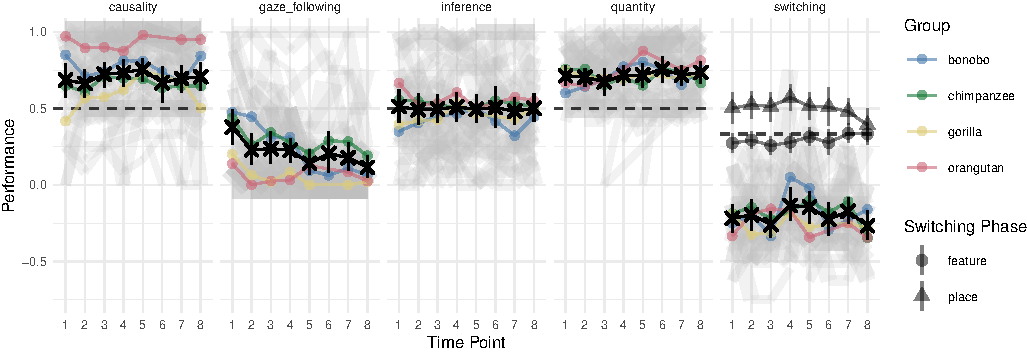
\includegraphics{figs/perfplot-1} 

}

\caption[Results from the five cognitive tasks across time points]{Results from the five cognitive tasks across time points. Black crosses show mean performance at each time point across species (with 95\% CI). Colored dots show mean performance by species. Transparent grey lines connect individual performances across time points, with the size of the line corresponding to the number of participants. Dashed line shows the chance level whenever applicable. The panel for switching includes triangles and dots showing the mean performance in the two phases from which the overall performance score was computed (see main text).}\label{fig:perfplot}
\end{figure*}
\end{CodeChunk}

\hypertarget{methods}{%
\section{Methods}\label{methods}}

\hypertarget{participants}{%
\subsection{Participants}\label{participants}}

A total of 40 great apes participated at least once in one of the tasks.
This included 8 Bonobos (3 females, age 7.3 to 38), 21 Chimpanzees (16
females, age 2.6 to 54.9), 6 Gorillas (4 females, age 2.7 to 21.6) and ,
6 Orangutans (4 females, age 17 to 40.2). The sample size at the
different time points ranged from 22 to 38.

Apes were housed at the Wolfgang Köhler Primate Research Center, located
at Zoo Leipzig in Leipzig, Germany. They live in groups, with one group
per species and two chimpanzee groups. Research was noninvasive and
strictly adhered to the legal requirements in Germany. Animal husbandry
and research complied with the European Association of Zoos and Aquaria
Minimum Standards for the Accommodation and Care of Animals in Zoos and
Aquaria as well as the World Association of Zoos and Aquariums Ethical
Guidelines for the Conduct of Research on Animals by Zoos and Aquariums.
Participation was voluntary, all food was given in addition to the daily
diet, and water was available ad libitum throughout the study. The study
was approved by an internal ethics committee at the Max Planck Institute
for Evolutionary Anthropology.

\hypertarget{design-setup-and-procedure}{%
\subsection{Design, Setup and
Procedure}\label{design-setup-and-procedure}}

\begin{CodeChunk}
\begin{figure*}[h]

{\centering 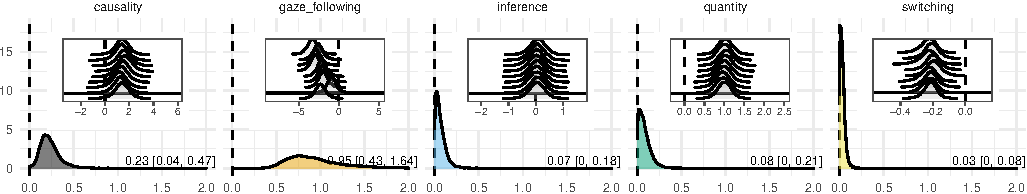
\includegraphics{figs/metaplot-1} 

}

\caption[Posterior distributions for $\tau$ from the meta-analytic models for each task]{Posterior distributions for $\tau$ from the meta-analytic models for each task. Numbers denote mean and 95\% HDI for $\tau$. Insets show the posterior distribution for the model intercept estimate at each time point and the overall estimate at the bottom (separated by the black line).}\label{fig:metaplot}
\end{figure*}
\end{CodeChunk}

We tested apes on the same five tasks every other week. Here we report
the data from the first eight time points. The tasks were presented in
the same order and with the same positioning and counterbalancing (to
keep conditions constant between individuals and across occasions). Apes
were tested in familiar sleeping or observation rooms by a single
experimenter. Whenever possible, they were tested individually. For each
individual, the tasks at one time point were usually spread out across
two consecutive days with causality and inference on day 1 and quantity
and switching on day 2. Gaze following trials were run at the beginning
and the end of each day. The basic setup comprised a sliding table
positioned in front of a clear Plexiglas panel. The experimenter sat on
a small stool and used an occluder to cover the sliding table.

\hypertarget{causality}{%
\subsubsection{Causality}\label{causality}}

The causality and inference tasks were modeled after (Call, 2004). Two
identical cups with a lid were placed left and right on the table. The
experimenter covered the table with the occluder, retrieved a piece of
food and hid it in one the cups outside the view of the participant.
Next, they removed the occluder, picked up the baited up and shook it
three times, which produced a rattling sound. Next the cup was put back
in place, the sliding table pushed forwards and the participant made a
choice by pointing to one of the cups. If they picked the baited cup,
there choice was coded as correct and they received the reward. On each
time point, participants received 12 trials.

\hypertarget{inference-by-exclusion}{%
\subsubsection{Inference by Exclusion}\label{inference-by-exclusion}}

Inference trials were identical to causality trials but instead of
shaking the baited cup, the experimenter shook the empty cup. On each
time point, participants received 12 trials. Inference trials were
intermixed with causality trials.

\hypertarget{gaze-following}{%
\subsubsection{Gaze Following}\label{gaze-following}}

The gaze following task was modeled after (Brauer, Call, \& Tomasello,
2005). The experimenter sat opposite the ape and handed over food at a
constant pace. That is, the experimenter picked up a piece of food,
briefly held it out in front of her face and then handed it over to the
participant. At some point, the experimenter looked up (i.e.~moving her
head up) while holding up the food in front of her head. After 10s, the
experimenter looked down again and handed over the food. We coded
whether the subject looked up during the 10s interval. Participants
received a total of 8 trials, spread out across the two test days.

\hypertarget{quantity-discrimination}{%
\subsubsection{Quantity Discrimination}\label{quantity-discrimination}}

For this task, we followed the general procedure of (Hanus \& Call,
2007). Two small plates were presented left and right on the table. The
experimenter placed 5 small food pieces on one plate and 7 in the other.
Then they pushed the sliding table forwards, and the subject made a
choice. We coded as correct when the subject chose the plate with the
larger quantity. There were 12 trials per time point.

\hypertarget{switching}{%
\subsubsection{Switching}\label{switching}}

This task was modeled after (Haun, Call, Janzen, \& Levinson, 2006).
Three different looking cups (silver cup with handle, plastic ice cone,
red cup without handle) were placed next to each other on the table.
There were two condition, in the place condition, the experimenter hid a
piece of food under one of the cups in full view of the participant.
Next, the cups were covered by the occluder and the experimenter
switched the position of two cups, while the reward remained in the same
location. We coded as correct, if the participant chose the location
where the food was hidden. Participants received four trials in this
condition. The feature condition, followed the same procedure but now
the experimenter also moved the reward when switching the cups. A
correct choice in this condition meant choosing the location that the
cup was moved to. Here, participants received 8 trials. The dependent
measure of interest for this task was calculated as:
\texttt{{[}proportion\ correct\ place{]}\ -\ (1\ -\ {[}proportion\ correct\ feature{]})}.
Positive values in this score mean that participants were quickly able
to switch between choosing based on location to choosing based on
feature. High negative values suggest that participants did not switch
strategies.

\hypertarget{analysis-and-results}{%
\section{Analysis and Results}\label{analysis-and-results}}

We combined the data from all species for the analysis because sample
sizes for some species were too small to get representative estimates.
However, we accounted for the nesting of subjects in species as part of
the random effect structure of our models. All analysis were run in
\texttt{R} (R Core Team, 2018). Bayesian multilevel models were
implemented using the package \texttt{brms} (Burkner, 2017) and used
default priors. All models included random intercepts for participants
nested within group and random slopes for trial
(\texttt{trial\textbar{}group/subject}). Data and analysis code can be
found in the associate online repository (see below).

\hypertarget{stability}{%
\subsection{Stability}\label{stability}}

First we looked at group level stability in performance. That is, we
asked how much performance varied across time points in the different
tasks. For this analysis, we ignored the temporal order of the different
time points and treated them as repetitions of the same experiment
(i.e.~time point was treated as a factor instead of a numerical
variable). As such, we asked a meta-analytic question: how much
variation is there between different instances of the same experiment.
To answer this, we fitted a mixed model with a random intercept term for
time point to the data from each task\footnote{We modeled the trial by
  trial data using a binomial distribution in a logistic GLMM for all
  tasks, except switching. Here we modeled the score (by time point) as
  a truncated normal distribution. As mentioned above, these models
  included random intercept terms for individuals nested within groups}.
As part of each model, we estimated a standard deviation of the random
intercept term (\(\tau\)), which reflects the variation between time
points.

Figure \ref{fig:perfplot} visualizes performance across time points. For
causality, inference and quantity, we can evaluate group level
performance by comparing it to chance (50\% correct = intercept of 0 in
link space). Group level performance was reliably above chance for
causality and quantity but at chance for quantity. For gaze following,
there is no such reference level and we can simply say that at at least
some individuals of all species followed the experimenter's gaze. The
switching score was consistently negative, suggesting that - on a group
level - apes did not switch strategies.

Figure \ref{fig:metaplot} shows the posterior distribution of \(\tau\)
for each task. While performance was very stable for inference, quantity
and switching (\(\tau\) very close to 0), performance was slightly more
variable for causality and varied substantially for gaze following. For
causality, variation did not seem to follow a clear temporal pattern. On
the other hand, for gaze following, there seems to be a downward trend
with apes (as a group) becoming less likely to follow the experimenter's
gaze. We explore this temporal pattern in more detail below. Taken
together, we may say that 4 out of 5 measures yield stable measures of
group level performance.

\hypertarget{reliability}{%
\subsection{Reliability}\label{reliability}}

Next, we asked how stable performance is on an individual level. This
question also relates to the reliability of each task - how well suited
it is to capture differences between individuals. In general,
reliability is high if individuals are consistently ranked across
measurement instances. One way to assess reliability is to correlate
performance from two time points (re-test reliability). Because we had
multiple time points, we computed pairwise correlations for all
combinations of time points (total of 28 unique correlations per task).
This results in a distribution of correlations, which we visualize in
Figure \ref{fig:relplot}. Results suggest good re-test reliability for
gaze following, causality and inference, variable reliability for
quantity and poor reliability for switching. This pattern is interesting
in light of the group level performance we reported above: stable
performance on a group level does not imply stable individual
differences. We come back to this point in the discussion.

\begin{CodeChunk}
\begin{figure}[H]

{\centering 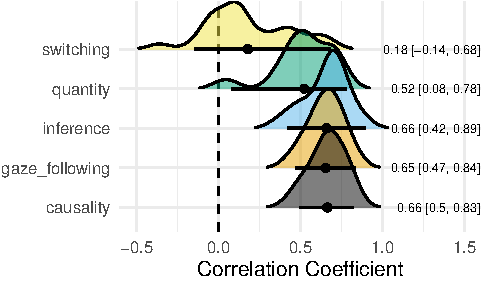
\includegraphics{figs/relplot-1} 

}

\caption[Distribution of correlations between time points for each task]{Distribution of correlations between time points for each task. Dots represent the mean of the distribution with 95\% HDI. Numbers denote mean and 95\% HDI.}\label{fig:relplot}
\end{figure}
\end{CodeChunk}

\hypertarget{predictors}{%
\subsection{Predictors}\label{predictors}}

In the final set of analysis, we investigated if variation in cognitive
performance could -- in part -- be explained by participant
characteristics. We chose to look at variables that are commonly
analyzed in the primate cognition literature: age, sex, rank and rearing
history. Rank was rated by animal keepers at every time point and
rearing history was classified as ``mother reared'', ``human reared''
and ``unknown''.

For each task, we ran the same five models\footnote{We used the same
  response distributions as in the stability analysis.}: A baseline
model predicting performance by time point (numerical) and trial as well
as four models, each with one of the predictors (age, sex, rank and
rearing history) added to the baseline model. We did not investigate any
interaction models (interactions among the predictors or with time
point) because we had no specific hypothesis in that direction. We used
Bayesian model comparison based on WAIC (widely applicable information
criterion) scores and weights (McElreath, 2016). This comparison tells
us which of the models considered makes the best out-of-sample
predictions. If the model with one predictor (e.g.~age) would be
consistently assigned the highest weight across tasks, we would conclude
that cognitive performance is best predicted by participants' age.

Table 1 gives WAIC scores and weights for each model and task. Figure
\ref{fig:predplot} shows the posterior distribution of the test
predictors (as well as for time point). The baseline model was ranked
highest across tasks (first or second for all tasks), suggesting that
none of the test predictors was consistently related to performance.
Within the baseline model, the estimate for time point was close to 0
for all tasks except gaze following, for which it was largely negative
(reflecting the downward trend we saw in Figure \ref{fig:perfplot}).

For gaze following, the model including sex as predictor was ranked
highest: males were somewhat less likely to follow the experimenter's
gaze. For quantity and witching, the rank model was rated highest with
lower ranking individuals showing better quantity discrimination or
switching abilities. In the case of switching, the model results should
be interpreted with caution. The low re-test correlations suggests that
the task does not reliably measure the cognitive ability in question.
Thus, the variation in performance that the model tries to explain might
not have a cognitive origin and could equally well be due to factors we
did not capture.

\begin{CodeChunk}
\begin{figure*}[h]

{\centering 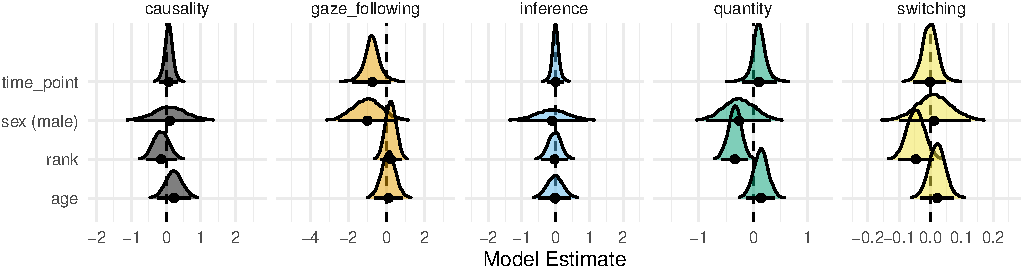
\includegraphics{figs/predplot-1} 

}

\caption[Posterior distribution for the test predictors for each task]{Posterior distribution for the test predictors for each task. Dots represent the mean of the distribution with 95\% HDI. Samples for time point are drawn from the baseline model. For all models except switching, the estimates are given in link space. No samples are shown for the rearing model because the factor had three levels and the model was ranked lowest for all tasks.}\label{fig:predplot}
\end{figure*}
\end{CodeChunk}

\hypertarget{discussion}{%
\section{Discussion}\label{discussion}}

We tested the same sample of great apes repeatedly on five cognitive
tasks. This design allowed us to address some pressing questions in
primate cognition research: How stable is group level performance in
cognitive tasks? How reliable are the results of these tasks? How much
is performance influenced by individual characteristics? Below we
discuss the results in light of these questions.

Performance was relatively stable for all tasks except gaze following.
This result is somewhat surprising given that individuals were
differentialy reinforced in all tasks -- except gaze following.
Furthermore, counterbalancing and positioning were exactly the same at
each time point. Together, this creates a scenario that would be ideal
for learning effects. How can we interpret this lack of improvement? One
interpretation could be that the different routes to solving the task
constitute incompatible information sources for great apes. For example,
in the case of causality, apes could solve the task by spontaneously
inferring that the sound was caused by the food. Alternatively, they
could learn that whenever they hear a rattling sound, food is under the
cup the experimenter touches. In principle, these two information
sources could easily be integrated and supplement one another -
resulting in an improvement of performance over time. The absence of
improvement could mean that apes rely on spontaneous inferences alone.
However, many alternative explanation are possible. For example, many of
the apes in Leipzig Zoo have had years of experience with the kind of
tasks we included in the study. Thus, the absence of improvement might
indicated that they already reached an individual performance maximum.
the continuation of this project might help to shed light on these
questions. For now, we may conclude that short term improvements based
on learned arbitrary relations are unlikely to occur in great apes. In
support of this interpretation, when researchers want primates to learn
arbitrary relations, it takes a very long time and an elaborate training
regime (e.g.~Allritz, Call, \& Borkenau, 2016; Vasconcelos, 2008).

Three out of five tasks showed acceptable levels of reliability.
Importantly, reliability is independent from group level performance
(leaving aside floor and ceiling effects) (see Hedge, Powell, \& Sumner,
2018). Here, we see such a pattern for inference: Group level
performance was consistently at chance level for every time point. On a
group level, one would conclude that great apes did not make the
inference in question. However, the tasks was highly reliable,
suggesting that it accurately captured individual differences. Together
with the observation that some individuals consistently performed at
ceiling (see grey transparent lines in Figure \ref{fig:perfplot}), this
suggests that the task is well suited to measure inferential abilities
on a \emph{individual} level. The opposite pattern holds for quantity.
Here, group level performance was consistently above chance but
individual differences were not very consistent. This suggests that
variation was due to sources other than systematic differences between
individuals. This phenomenon is quite common in the adult cognitive
literature {[}hedge2018reliability{]} and arises when experimental tasks
(optimized for low variance in measurement) are used to study individual
differences (requiring high variance in measurement). Taken together, we
may recommend that researchers select their tasks depending on the kind
of questions they want to answer. When planning to study individual
differences by relating measures to one another, researchers are well
advised to first study the reliability of these measures. Even though
this takes considerable time and effort, it increases to the chances of
finding effects.

\begin{table}[H]
\centering
\begin{tabular}{rllrrr}
  \hline
 & Task & Model & WAIC & SE & Weight \\ 
  \hline
1 & Causality & baseline & 2432.35 & 52.98 & 0.25 \\ 
  2 &  & rank & 2432.80 & 53.03 & 0.20 \\ 
  3 &  & age & 2433.05 & 53.09 & 0.18 \\ 
  4 &  & sex & 2432.56 & 53.07 & 0.23 \\ 
  5 &  & rearing & 2433.45 & 53.09 & 0.15 \\ 
  6 & Gaze following & baseline & 1133.68 & 50.19 & 0.22 \\ 
  7 &  & rank & 1134.56 & 50.26 & 0.14 \\ 
  8 &  & age & 1134.31 & 50.29 & 0.16 \\ 
  9 &  & sex & 1132.74 & 50.19 & 0.35 \\ 
  10 &  & rearing & 1134.65 & 50.41 & 0.13 \\ 
  11 & Inference & baseline & 2915.33 & 44.01 & 0.24 \\ 
  12 &  & rank & 2916.23 & 44.03 & 0.16 \\ 
  13 &  & age & 2915.98 & 44.07 & 0.18 \\ 
  14 &  & sex & 2915.19 & 44.13 & 0.26 \\ 
  15 &  & rearing & 2916.17 & 44.20 & 0.16 \\ 
  16 & Quantity & baseline & 2501.47 & 47.63 & 0.23 \\ 
  17 &  & rank & 2500.65 & 47.74 & 0.35 \\ 
  18 &  & age & 2502.04 & 47.73 & 0.18 \\ 
  19 &  & sex & 2502.54 & 47.70 & 0.14 \\ 
  20 &  & rearing & 2503.18 & 47.75 & 0.10 \\ 
  21 & Switching & baseline & 25.56 & 22.13 & 0.30 \\ 
  22 &  & rank & 25.12 & 21.94 & 0.37 \\ 
  23 &  & age & 27.20 & 22.27 & 0.13 \\ 
  24 &  & sex & 27.19 & 22.14 & 0.13 \\ 
  25 &  & rearing & 28.41 & 22.31 & 0.07 \\ 
   \hline
\end{tabular}
\caption{WAIC Scores and weights for each predictor model and task.} 
\end{table}

We did not find that one of the individual level characteristics (age,
sex, rank or rearing history) was consistently related to performance
across tasks. A baseline model, predicting performance by time variables
alone was, on average, rated highest in the different model comparisons.
The model including rank was rated highest for two tasks (quantity and
switching). However, in the case of switching, this should be
interpreted with caution in the light of low reliability of the task
(see results section). Moving forward, we will explore additional
predictors, to see if we do find some that are related to cognitive
performance more broadly. For now, we may conclude that researchers
should carefully select predictors based on theoretical considerations.
Including them as a default or to control for potential effects might
make models unnecessarily complex -- and might not even have the desired
effect (see Westfall \& Yarkoni, 2016).

For our analysis, we combined the data from all species, neglecting
potential species differences. The reason is simply that the sample size
for each species was too small to really differentiate individual from
species level differences. This is a common problem in primate cognition
research. Species level inferences require data sets that are beyond the
resources of individual labs. A promising way forward to overcome this
limitation is the \emph{ManyPrimates} project; a large-scale
collaborative initiative initiated to establish and infrastructure to
support the pooling of resources across labs (ManyPrimates, Altschul,
Beran, Bohn, Call, et al., 2019).

The data we have reported here are the first couple of waves in a
lonitudinal study which we hope to continue for at least one year. As
part of it, we will record additional variables that might help to
explain variation in cognitive performance such as social network data
or live history variables (sickness, birth and death of group members,
etc.). We hope that this project will contribute to our understanding of
the dynamic nature of primate cognition.

\vspace{1em}

\fbox{\parbox[b][][c]{7.3cm}{\centering Corresponding data and code are available at\ \url{https://github.com/ccp-eva/laac}}}
\vspace{1em}

\hypertarget{acknowledgements}{%
\section{Acknowledgements}\label{acknowledgements}}

Masked for peer review

\hypertarget{references}{%
\section{References}\label{references}}

\setlength{\parindent}{-0.1in} 
\setlength{\leftskip}{0.125in}

\noindent

\hypertarget{refs}{}
\leavevmode\hypertarget{ref-allritz2016chimpanzees}{}%
Allritz, M., Call, J., \& Borkenau, P. (2016). How chimpanzees (pan
troglodytes) perform in a modified emotional stroop task. \emph{Animal
Cognition}, \emph{19}(3), 435--449.

\leavevmode\hypertarget{ref-brauer2005all}{}%
Brauer, J., Call, J., \& Tomasello, M. (2005). All great ape species
follow gaze to distant locations and around barriers. \emph{Journal of
Comparative Psychology}, \emph{119}(2), 145.

\leavevmode\hypertarget{ref-R-brms_a}{}%
Burkner, P.-C. (2017). brms: An R package for Bayesian multilevel models
using Stan. \emph{Journal of Statistical Software}, \emph{80}(1), 1--28.

\leavevmode\hypertarget{ref-call2004inferences}{}%
Call, J. (2004). Inferences about the location of food in the great apes
(pan paniscus, pan troglodytes, gorilla gorilla, and pongo pygmaeus).
\emph{Journal of Comparative Psychology}, \emph{118}(2), 232.

\leavevmode\hypertarget{ref-open2015estimating}{}%
Collaboration, O. S. (2015). Estimating the reproducibility of
psychological science. \emph{Science}, \emph{349}(6251).

\leavevmode\hypertarget{ref-farrar2020replicomp}{}%
Farrar, B. G., Boeckle, M., \& Clayton, N. S. (2020). Replications in
comparative cognition: What should we expect and how can we improve?
\emph{Animal Behavior and Cognition}, \emph{7}(1), 1.

\leavevmode\hypertarget{ref-farrar2020replications}{}%
Farrar, B., Voudouris, K., \& Clayton, N. (2020). Replications,
comparisons, sampling and the problem of representativeness in animal
behavior and cognition research.

\leavevmode\hypertarget{ref-hanus2007discrete}{}%
Hanus, D., \& Call, J. (2007). Discrete quantity judgments in the great
apes (pan paniscus, pan troglodytes, gorilla gorilla, pongo pygmaeus):
The effect of presenting whole sets versus item-by-item. \emph{Journal
of Comparative Psychology}, \emph{121}(3), 241.

\leavevmode\hypertarget{ref-haun2006evolutionary}{}%
Haun, D. B., Call, J., Janzen, G., \& Levinson, S. C. (2006).
Evolutionary psychology of spatial representations in the hominidae.
\emph{Current Biology}, \emph{16}(17), 1736--1740.

\leavevmode\hypertarget{ref-hedge2018reliability}{}%
Hedge, C., Powell, G., \& Sumner, P. (2018). The reliability paradox:
Why robust cognitive tasks do not produce reliable individual
differences. \emph{Behavior Research Methods}, \emph{50}(3), 1166--1186.

\leavevmode\hypertarget{ref-many2019establishing}{}%
ManyPrimates, Altschul, D. M., Beran, M. J., Bohn, M., Call, J., DeTroy,
S., \ldots{} others. (2019). Establishing an infrastructure for
collaboration in primate cognition research. \emph{PLoS One},
\emph{14}(10), e0223675.

\leavevmode\hypertarget{ref-primates2019collaborative}{}%
ManyPrimates, Altschul, D. M., Beran, M. J., Bohn, M., Caspar, K. R.,
Fichtel, C., \ldots{} others. (2019). Collaborative open science as a
way to reproducibility and new insights in primate cognition research.
\emph{Japanese Psychological Review}, \emph{62}(103), 205--220.

\leavevmode\hypertarget{ref-rethinking}{}%
McElreath, R. (2016). \emph{Statistical rethinking: A bayesian course
with examples in R and Stan} (pp. xvii, 469). Boca Raton: CRC Press.

\leavevmode\hypertarget{ref-R-base}{}%
R Core Team. (2018). \emph{R: A language and environment for statistical
computing}. Vienna, Austria: R Foundation for Statistical Computing.

\leavevmode\hypertarget{ref-shaw2017cognitive}{}%
Shaw, R. C., \& Schmelz, M. (2017). Cognitive test batteries in animal
cognition research: Evaluating the past, present and future of
comparative psychometrics. \emph{Animal Cognition}, \emph{20}(6),
1003--1018.

\leavevmode\hypertarget{ref-simmons2011false}{}%
Simmons, J. P., Nelson, L. D., \& Simonsohn, U. (2011). False-positive
psychology: Undisclosed flexibility in data collection and analysis
allows presenting anything as significant. \emph{Psychological Science},
\emph{22}(11), 1359--1366.

\leavevmode\hypertarget{ref-stevens2017replicability}{}%
Stevens, J. R. (2017). Replicability and reproducibility in comparative
psychology. \emph{Frontiers in Psychology}, \emph{8}, 862.

\leavevmode\hypertarget{ref-vasconcelos2008transitive}{}%
Vasconcelos, M. (2008). Transitive inference in non-human animals: An
empirical and theoretical analysis. \emph{Behavioural Processes},
\emph{78}(3), 313--334.

\leavevmode\hypertarget{ref-volter2018comparative}{}%
Volter, C. J., Tinklenberg, B., Call, J., \& Seed, A. M. (2018).
Comparative psychometrics: Establishing what differs is central to
understanding what evolves. \emph{Philosophical Transactions of the
Royal Society B: Biological Sciences}, \emph{373}(1756), 20170283.

\leavevmode\hypertarget{ref-westfall2016statistically}{}%
Westfall, J., \& Yarkoni, T. (2016). Statistically controlling for
confounding constructs is harder than you think. \emph{PloS One},
\emph{11}(3), e0152719.

\bibliographystyle{apacite}


\end{document}
